\section{Khám phá: lệch bao nhiêu, ở tháng nào, kênh nào}

\subsection{Theo tháng}

\begin{figure}[H]
\centering
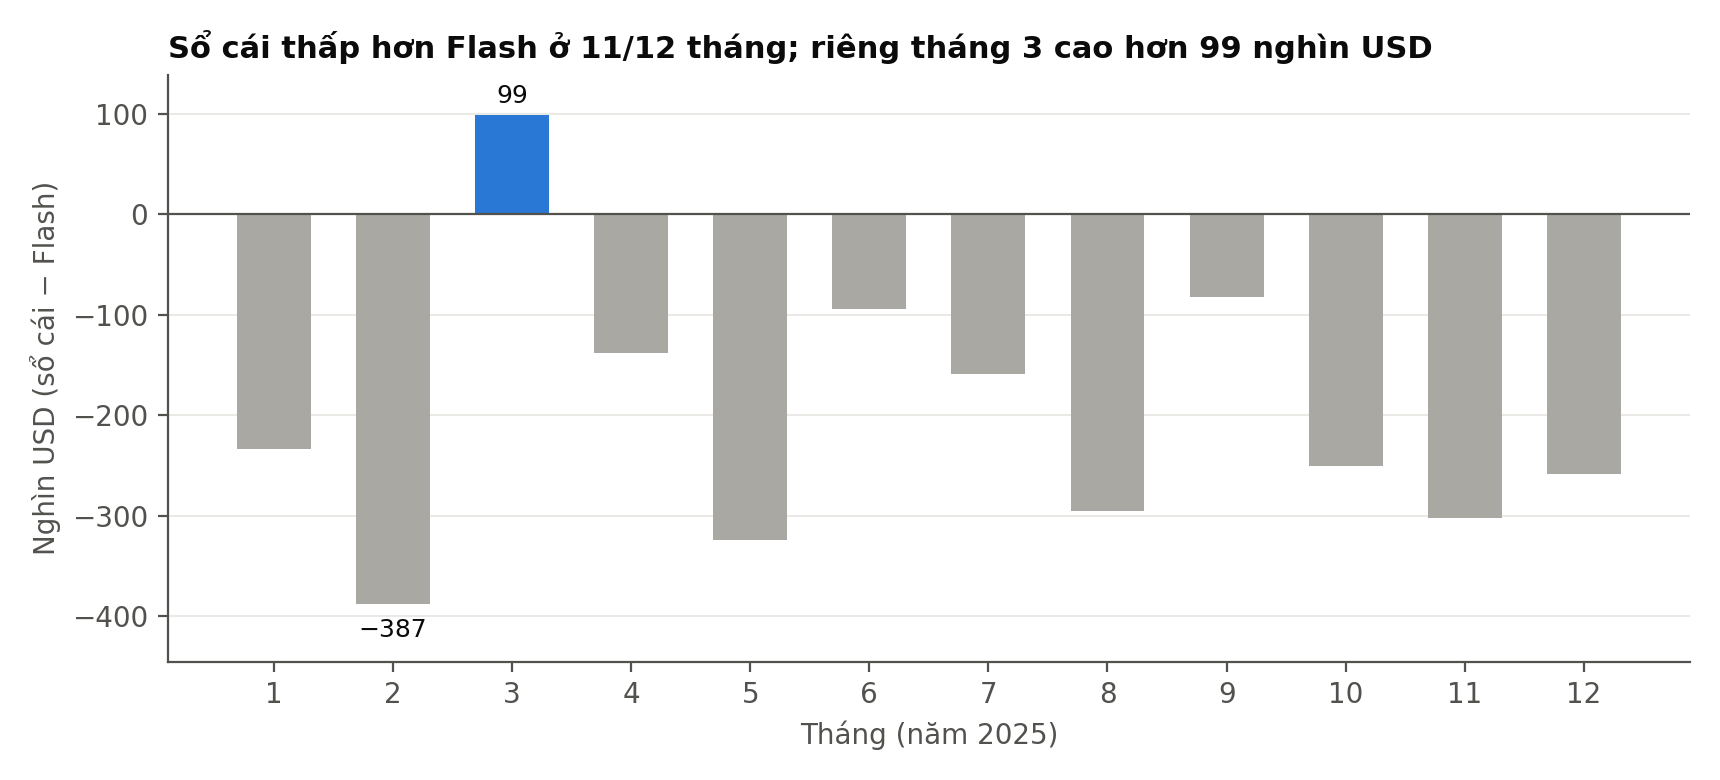
\includegraphics[width=0.95\textwidth]{generated/hinh_chenh_lech_thang.png}

\capfig{Chênh lệch sổ cái $-$ Flash theo tháng, nghìn USD \nguon{BR-Tổng}.}\label{fig:thang}
\end{figure}

Sổ cái thấp hơn Flash ở \SoThangThap{}/12 tháng (Hình~\ref{fig:thang}, Bảng~\ref{tab:thang}). Ba điểm cần giải thích ở phần sau:
\begin{itemize}
  \item \textbf{Tháng 3 đi ngược chiều}: sổ cái cao hơn Flash \SoThangBaChenhLech{} USD (+\SoThangBaPct). Nếu chênh lệch chỉ do chiết khấu và đơn hủy thì không tháng nào có thể dương, nên phải có một khoản theo thời điểm đẩy doanh thu vào tháng 3.
  \item \textbf{Mức lệch dao động mạnh} giữa các tháng: nặng nhất theo \% là \SoThangLechNhatPct{}, nặng nhất theo số tiền là \SoThangLechNhatTien{} USD.
  \item Chênh lệch cả năm là \SoChenhLechNam{} USD (\SoPctNam{} so với Flash).
\end{itemize}

\begin{table}[H]
\captab{Flash, sổ cái và chênh lệch theo tháng, USD \nguon{BR-Tổng}}\label{tab:thang}
\centering
\begin{tabular}{@{}l r r r r@{}}
\toprule
Tháng & Flash & Sổ cái & Chênh lệch & \% so với Flash \\
\midrule
Tháng 1 & 2.859.589 & 2.626.167,29 & $-$233.421,71 & $-$8,16\% \\
Tháng 2 & 3.490.159 & 3.102.906,99 & $-$387.252,01 & $-$11,10\% \\
Tháng 3 & 2.001.911 & 2.100.928,53 & 99.017,53 & 4,95\% \\
Tháng 4 & 1.035.907 & 898.049,36 & $-$137.857,64 & $-$13,31\% \\
Tháng 5 & 2.802.769 & 2.478.745,50 & $-$324.023,50 & $-$11,56\% \\
Tháng 6 & 2.506.912 & 2.412.461,84 & $-$94.450,16 & $-$3,77\% \\
Tháng 7 & 2.248.805 & 2.089.895,01 & $-$158.909,99 & $-$7,07\% \\
Tháng 8 & 2.569.740 & 2.274.164,62 & $-$295.575,38 & $-$11,50\% \\
Tháng 9 & 2.576.818 & 2.494.221,48 & $-$82.596,52 & $-$3,21\% \\
Tháng 10 & 2.743.824 & 2.493.635,92 & $-$250.188,08 & $-$9,12\% \\
Tháng 11 & 2.806.714 & 2.504.559,28 & $-$302.154,72 & $-$10,77\% \\
Tháng 12 & 3.481.253 & 3.222.760,41 & $-$258.492,59 & $-$7,43\% \\
\midrule
\textbf{Cả năm} & \textbf{31.124.401} & \textbf{28.698.496,23} & \textbf{$-$2.425.904,77} & \textbf{$-$7,79\%} \\
\bottomrule
\end{tabular}

\end{table}

\subsection{Theo kênh}

\begin{table}[H]
\captab{Flash, sổ cái và chênh lệch theo kênh cả năm, USD \nguon{BR-CH}, \nguon{BR-WEB}}\label{tab:kenh}
\centering
\begin{tabular}{@{}l r r r r@{}}
\toprule
Kênh & Flash & Sổ cái & Chênh lệch & \% so với Flash \\
\midrule
Cửa hàng & 14.060.500 & 13.181.898,25 & $-$878.601,75 & $-$6,25\% \\
Online & 17.063.901 & 15.515.347,98 & $-$1.548.553,02 & $-$9,08\% \\
Chưa gắn kênh & 0 & 1.250,00 & 1.250,00 & -- \\
\midrule
\textbf{Tổng} & \textbf{31.124.401} & \textbf{28.698.496,23} & \textbf{$-$2.425.904,77} & \textbf{$-$7,79\%} \\
\multicolumn{3}{@{}l}{\textit{Kiểm tra: sổ cái cửa hàng + online $-$ tổng sổ cái}} & \textit{$-$1.250,00} & \\
\bottomrule
\end{tabular}

\end{table}

Kênh online chiếm \SoOnlineTyTrong{} phần chênh lệch (\SoOnlineChenhLech{} USD), nhiều hơn kênh cửa hàng, dù doanh số online chỉ hơn cửa hàng khoảng một phần năm. Dòng kiểm tra ở cuối Bảng~\ref{tab:kenh} cho thấy sổ cái của hai kênh cửa hàng và online cộng lại \textbf{thiếu \SoChuaGanKenh{} USD} so với tổng sổ cái: đó là bút toán ADJ-0925 không gắn kênh nào. Khoản này chỉ lộ ra khi kiểm tra các phần có cộng đủ tổng hay không.

\subsection{Điều chưa biết sau bước khám phá}

Bảng tổng chỉ trả lời "lệch bao nhiêu". Nó chưa trả lời lệch do đâu, phần nào hợp lệ, phần nào là lỗi, và vì sao tháng 3 đi ngược chiều. Mục~IV tách chênh lệch thành từng khoản, bắt đầu từ mức chi tiết nhất: cửa hàng $\times$ ngày và đơn online $\times$ ngày giao.
